\chapter{Design and implementation of a LoRa server}
\label{chap:server}

Since LoRaWAN was launched on the market a number of LoRa server has been released too. Most of them are presented as web services which provide the basic features of LoRaWAN for free, and in some case offering also some premium services. None of them, however, offers a complete control on the network, which is an essential requirement in order to completely explore the possibilities of this technology.

For these reasons it was decided to develop from scratch new LoRa server infrastructure, focusing in particular on designing a reliable tool which gives access to all information that can be extract from the behavior of the network. Moreover, having a complete custom software makes possible to make changes depending on the needs.

The goal of this work was to obtain a simple, yet flexible, software that can be adapted to different experimental condition without the of re-engineering a complex architecture. In other words, the solution which is presented in this chapter is not designed to be a competitor of the existing commercial network server.


\section{Architecture}
As is shown in figure \ref{fig:servercomponent}, the \emph{network server} and the \emph{application server} were designed to be two separate components, communicating through sockets. This choice follows the guidelines provided by Semtech, which are presented in section \ref{sec:loraservers}. Moreover, decoupling the two components makes possible to run them in different machines.

The communication with the gateway is done using the GWMP protocol presented in chapter \ref{chap:lorawan}, which makes this server immediately compatible with the majority of gateway present on the market.

\begin{figure}[]
\centering
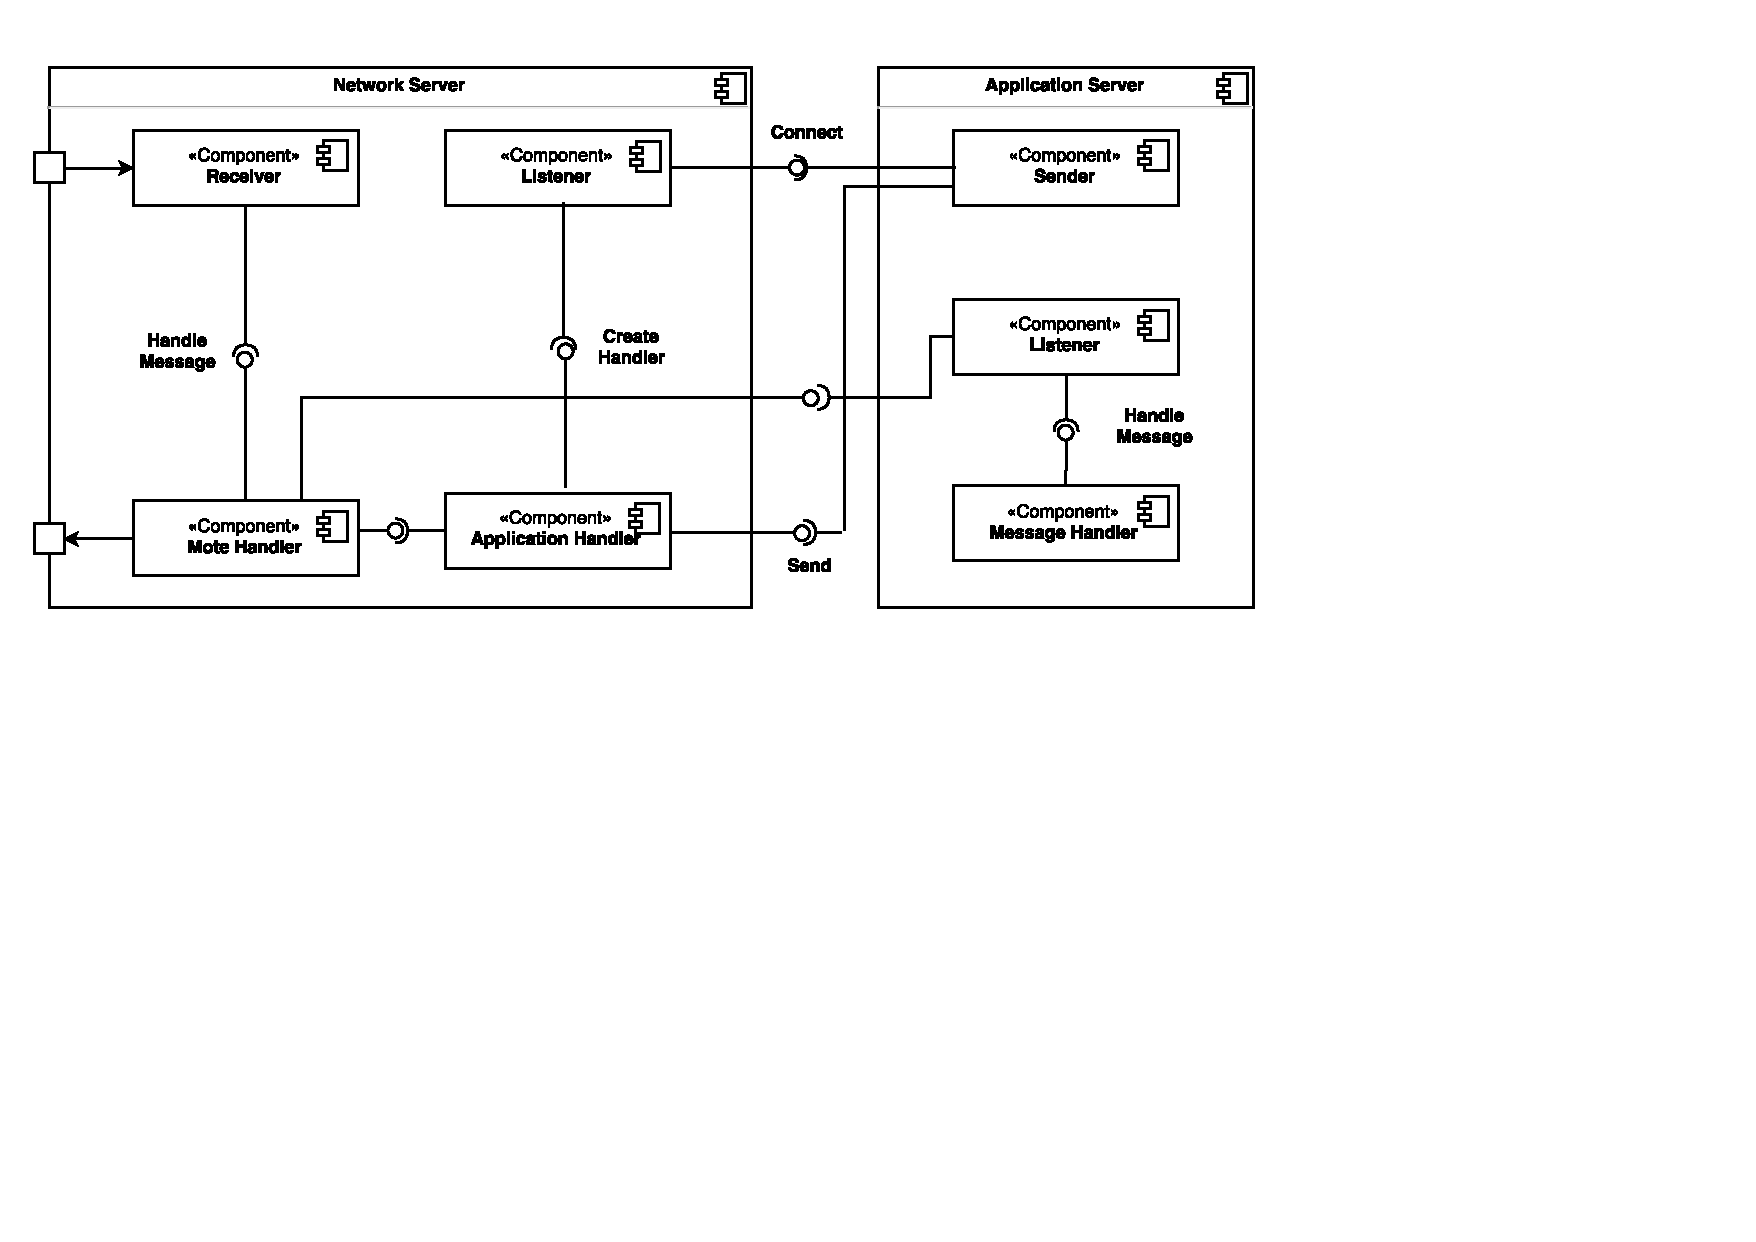
\includegraphics[width=\textwidth]{img/netserver}
\caption{Architecture of the network server}
\label{fig:servercomponent}
\end{figure}

\section{Network Server}
The network server consists of four separate components (figure \ref{fig:servercomponent}) which communicates among them by means of a set of shared data structure.

\subsubsection{Receiver}
The receiver component is responsible for receiving data from gateways trough to an UDP socket. If it receives a PULL\_DATA message, it stores address and port of the gateway in a dedicated data structure. In case of PUSH\_DATA, instead, it delivers the message to a pool of Mote Handler.

\subsubsection{Mote Handler}
The Mote Handler is charge of handling the message on a separate thread performing the following operations:

\begin{itemize}
\item it authenticates the frame by checking the MIC, and in case of failure it discards the message and terminates the execution;
\item it checks if the application server associated to the mote is connected to the network server and it forwards the user data to it;
\item it checks if there is a pending message to be sent to the mote; if the mote requested an acknowledgement by means of a \emph{Confirmed Data Up} message and there are no pending data, it sends back an empty message setting the ACK flag;
\item it updates the statistics of the correctly received message from the mote.
\end{itemize}


\subsubsection{Listener}
It waits for Application Servers that want to connect and creates an Application Handler for each one.

\subsubsection{Application Handler}
The Application Handler is responsible for receiving user data from the application server to which it is connected, and it pushes every received message to the pending queue of the corresponding mote.

\subsection{Implementation}
To obtain a platform independent product it was decided to implement it using the Java programming language, and in particular the Java 8 SDK. Since stability and reliability was a primary requirement the Network Server is implemented in a multi-thread fashion, so that every message is handled in a different thread. This choice brings greater robustness especially in unexpected situations because a wrong management of the message does not involve the malfunction of the entire server.

This multi-thread design is implemented by meas of the Java ExecutorService, in which a fixed pool of threads is created at start up and reused at run time.

In listing \ref{list:motehandler} the main function of each Mote Handler is shown. All data is stored in thread-safe data structures.

The Listener components implements the GWMP protocol to exchange data with gateways, while the MoteHandler parses uplink data and builds downlink messages on the basis of the LoRaWAN 1.0 specification.\cite{lorawanspec}

\begin{lstlisting}[caption=Main function of NetworkServerMoteHandler.java\label{list:motehandler}]
public void run() {
    if (message.getInt("stat") != 1) {
        activity.warning("CRC not valid, skip packet");
        return;
    }

    Packet packet = new Packet(message.getString("data"));

    switch (packet.type) {
        case Packet.JOIN_REQUEST:
            handleJoin(packet);
            break;
        case Packet.CONFIRMED_DATA_UP:
        case Packet.UNCONFIRMED_DATA_UP:
            handleMessage(packet);
            break;
        default:
            activity.warning("Message type not recognized");
    }
}
\end{lstlisting}
The most important function of the Mote Handler is the \texttt{handleMessage()}, reported in \ref{list:handlemsg}, which is in charge of handling the received packets, authenticating them and forwarding them to the Application Server. Since in class A LoRaWAN end-devices the receive windows are opened shortly after the upstream transmission, the first of which with the same parameters, the Mote Handler component must be responsible also for the correct transmission of the downstream messages. This operation is done in the \texttt{handleMessage()} by polling a frame from the queue of pending messages, and sending it to the gateway by means of the GWMP protocol.

\begin{lstlisting}[caption=Handle message in NetworkServerMoteHandler.java\label{list:handlemsg}]
private void handleMessage(Packet packet) {
    long timestamp = message.getLong("tmst");
    Frame fm = new Frame(packet);
    Mote mote = motes.get(fm.getDevAddress());

    if (mote == null) {
        activity.warning(fm.getDevAddress() + ": Mote not found");
        return;
    }

    // Authentication => check mic
    if (!packet.checkIntegrity(mote,fm.counter)) {
        activity.warning(fm.getDevAddress() + ": MIC not valid");
        return;
    }

    // Forward message to Application Server
    AppServer appServer = appServers.get(mote.getAppEUI());

    if (appServer == null) {
        activity.warning("App server NOT found");
    } else {
        String appserverMessage = buildAppserverMessage(gateway,message,packet.type,fm);
        try(Socket toAS = new Socket(appServer.address, appServer.port)) {
            PrintWriter out = new PrintWriter(new OutputStreamWriter(toAS.getOutputStream(), StandardCharsets.US_ASCII));
            out.println(appserverMessage);
            out.flush();
        } catch (IOException e) {
            e.printStackTrace();
        }
    }

    mote.updateStatistics(fm.counter); // Update mote statistics
    activity.info(mote.printStatistics());

    /*** SEND DOWNSTREAM MESSAGE ***/
    // Wait message to send
    String answer;
    try {
        answer = mote.messages.poll(TIMEOUT, TimeUnit.MILLISECONDS);
    } catch (InterruptedException e) {
        e.printStackTrace();
        return;
    }
    
    if (answer == null) {
        activity.info("Timeout, no message in queue to send to " + mote.getDevAddress());
        return;
    }

    Packet ansPacket = buildDownstreamMessage(answer, mote, (packet.type == Packet.CONFIRMED_DATA_UP));

    // If there there is one message in queue, send it
    GatewayMessage response = /* build response */
    try {
        socket.send(response.getPacket(gatewayAddr));
        activity.info("Sent message to mote: " + mote.getDevAddress());
    } catch (IOException e) {
        e.printStackTrace();
    }
}
\end{lstlisting}

\newpage
\section{Application Server}
The \emph{Application Server} includes three main components, as described by the component diagram in figure \ref{fig:servercomponent}.

\subsubsection{Sender}
The \emph{Sender} component is in charge of encrypt user data by means of the Application Session Key and it sends it to the Network Server. This component, and in general the overall application server, has no information on the timing constraint of the mote, so it sends the downstream message as soon they are produced. The correct scheduling of the messages into the correct receive window is done by the network server.

\subsubsection{Listener}
The \emph{Listener} component is responsible for waiting for the network server to connect and start the handler. It is designed to not interact with the received messages, but instead once the incoming connection is accepted and the socket is created the Listener starts the execution of the independent Handler component.

\subsubsection{Handler}
The \emph{Handler} is started by the Listener whenever the network server tries to connect, so it receives the upstream messages and decrypts it. It is the only component which receive data from the network server, so it is more error-prone than the other components due to potentially malformed incoming messages. For this reason the execution of each Handler must be independent from the other Handlers.

\subsection{Implementation}
As for the network server, also the application server was implemented in Java for exactly the same motivations. The multi-thread architecture is achieved by means of the Java ExecutorService, through which the handlers are executed, using a fixed pool of threads created at the start up.

In order to register with the network server, the first message sent by the Sender component to network server includes also the Application EUI of the application server and the listening address and port.

For the purposes of the experiments was developed a special Application Server Handler, able to keep track of the ongoing tests. It is possible to appreciate this extra feature in listing \ref{list:apphandler} at line 27 where the method \texttt{updateStatistics()} is invoked.


\begin{lstlisting}[caption=Main function of ApplicationServerHandler.java\label{list:apphandler}]
public void run() {
    while (true) {
        try {
            String message = socket.readLine();
            if(message == null) {
                return;
            }

            JSONObject m = new JSONObject(message);
            JSONObject appJson = m.getJSONObject("app");
            String moteEui = appJson.getString("moteeui");
            Mote mote = application.motes.get(moteEui);

            if (mote == null) {
                application.log.warning("Mote not found");
                continue;
            }

            JSONObject data = appJson.getJSONObject("userdata");
            int port = data.getInt("port");
            int seqno = data.getInt("seqno");
            byte[] ack = ByteBuffer.allocate(2).putShort((short) (seqno & 0xFFFF)).array();
            application.messages.add(new DownstreamMessage(mote, token++, 4, new String(Hex.encode(ack))));
            byte[] payload = decryptPayload(data.getString("payload"), mote, seqno);
            application.log.info(String.format("Received message from %s, port %d, counter %d",mote.getDevEUI(),port,seqno));
            messages.info(new String(Hex.encode(payload)));
            updateStitistics(mote, payload); // Analyze
        } catch (SocketException e) {
            if (e.getMessage().equals("Connection reset")){
                e.printStackTrace();
                return;
            }

        } catch (IOException e) {
            e.printStackTrace();
        }
    }
}
\end{lstlisting}
The decryption of the upstream data is done by the Handler component invoking the method \texttt{decryptPayload()}. This method, which is reported in listing \ref{list:decrypt}, implements the decryption of the payload exactly as described in the LoRaWAN specification. \cite{lorawanspec}

\begin{lstlisting}[caption=decryptPayload() in ApplicationServerHandler.java\label{list:decrypt}]
private byte[] decryptPayload(String payload, Mote mote, int counter) {
    if (payload == null || payload.length() == 0) {
        return new byte[0];
    }

    byte[] data = Base64.getDecoder().decode(payload.getBytes());
    int dataSize =  data.length;
    int targetSize = (dataSize % 16 == 0) ? dataSize : ((dataSize/16) + 1) * 16;

    ByteBuffer bb = ByteBuffer.allocate(targetSize).order(ByteOrder.LITTLE_ENDIAN);
    for (int i=1; i<=targetSize/16; i++) {
        bb.put((byte) 1);
        bb.putInt(0);
        bb.put(UPSTREAM_DIRECTION);
        bb.put(mote.devAddress);
        bb.putInt(counter);
        bb.put((byte) 0);
        bb.put((byte) i);
    }
    byte[] A = bb.array();
    byte[] decrypted = new byte[dataSize];

    try {
        // Create key and cipher
        Key aesKey = new SecretKeySpec(mote.appSessionKey, "AES");
        Cipher cipher = Cipher.getInstance("AES/ECB/NoPadding");

        // Create S
        cipher.init(Cipher.ENCRYPT_MODE, aesKey);
        byte[] S = cipher.doFinal(A);

        // Encryption
        for (int i=0; i<dataSize; i++) {
            decrypted[i] = (byte) (data[i] ^ S[i]);
        }
    } catch (Exception e) {
        e.printStackTrace();
    }
    return decrypted;
}
\end{lstlisting}
